
%\begin{center}

      \pagestyle{empty}


\fbox{
  \begin{minipage}[t][22.9cm]{16cm}  %% 24 cm
  \rule{0cm}{5mm}

  \vspace{-.7cm}
  \large  \hfill CEA DSM DAPNIA-02-395 (2002) \\[-.5cm]

  \vfill
  \vspace{-3cm}
  \title{ 
      \textbf{{\huge ZGOUBI USERS' GUIDE}     \\ 
           \textit{\large -- VERSION 4.3 --} }      \\
    }

    \author{ 
      \textbf{F. M\'eot } \\
         and       \\
      \textbf{S. Valero  }     \\
      { \em  CEA Saclay, DSM/DAPNIA/SEA,    }                       \\
      { \em F-91191 Gif-sur-Yvette Cedex, France }           
    }

    \maketitle
    \date

    \vfill

    \centerline{
      \mbox{
         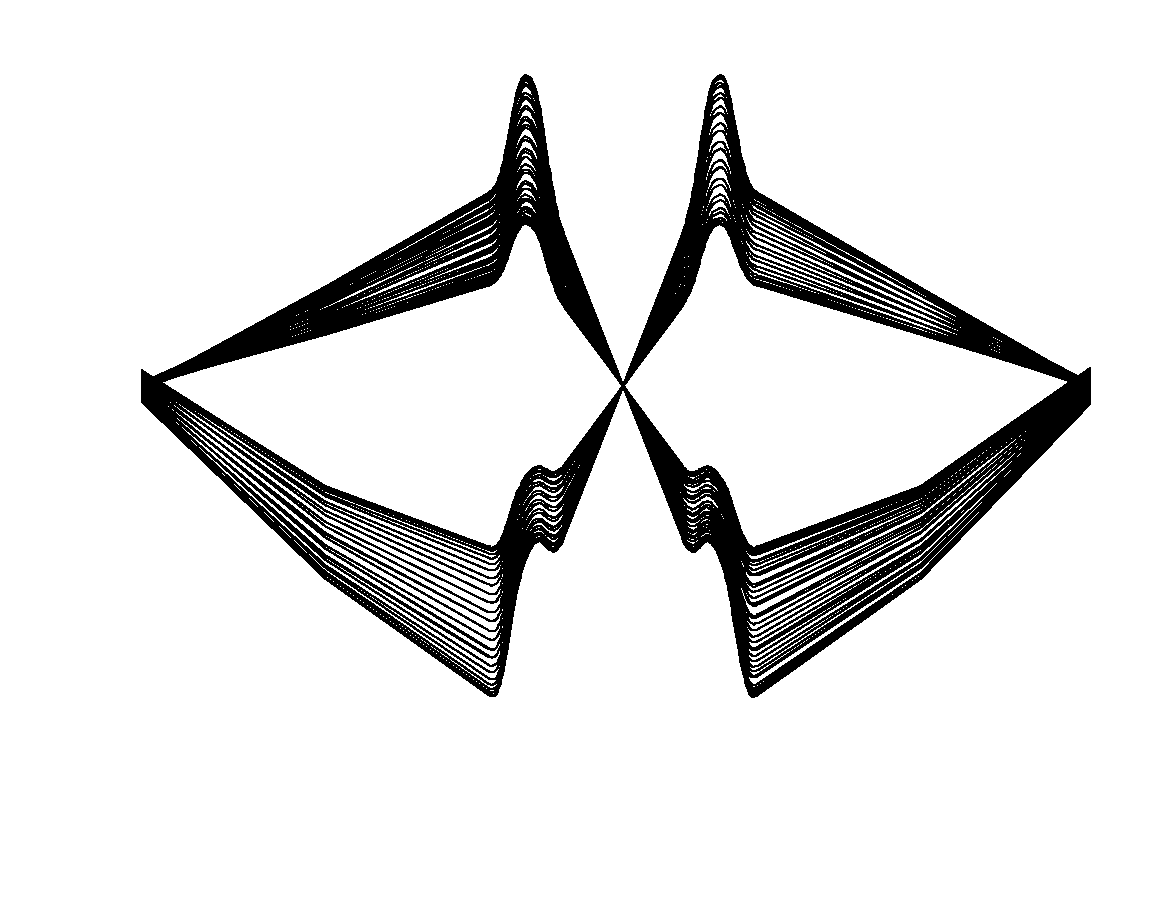
\includegraphics[width=7cm]{FigCover1.ps}
         \hfill
         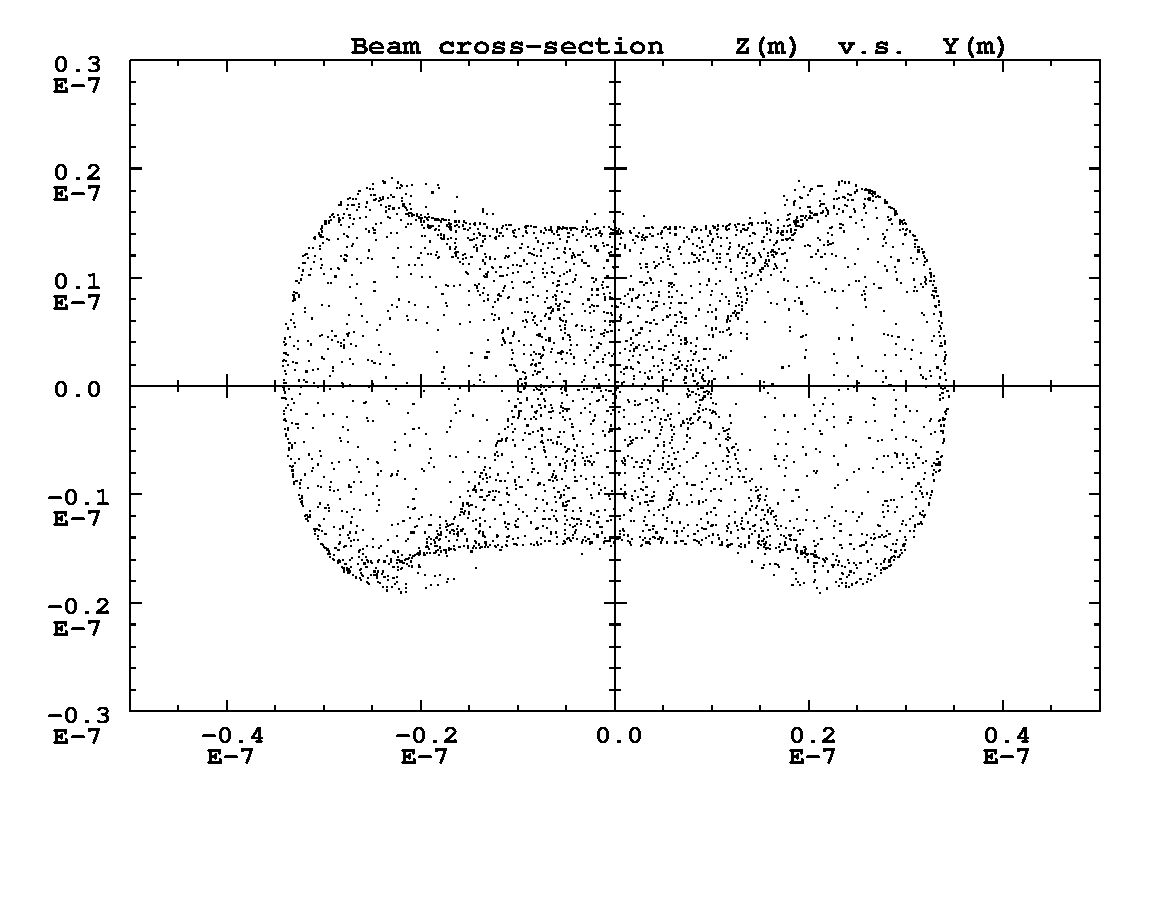
\includegraphics[width=7cm]{FigCover2.ps} \\
       }
     }

    \centerline{
      \mbox{
         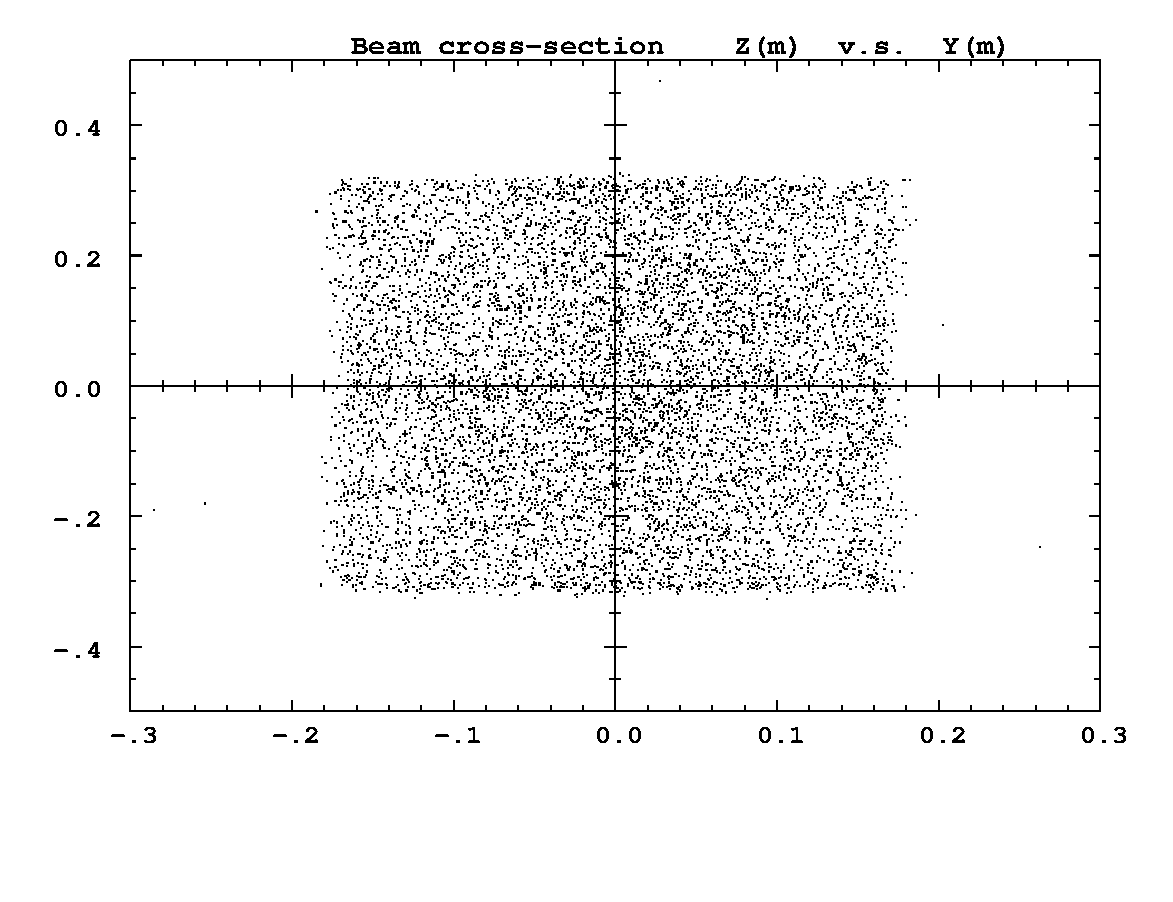
\includegraphics[width=7cm]{FigCover3.ps}
         \hfill
         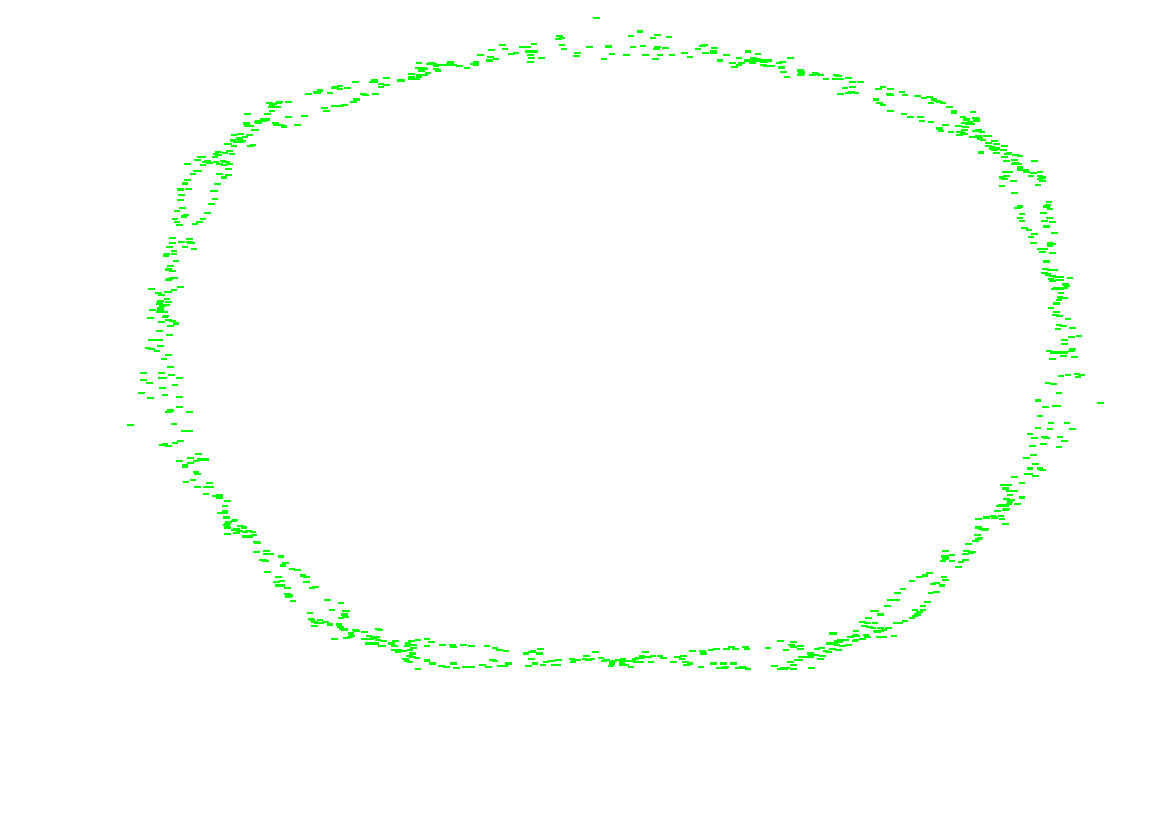
\includegraphics[width=7cm]{FigCover4.ps}
       }
     }

  \end{minipage}
}
%\end{center}


\newpage


~~~~~~~~~~~
  \footnotetext{\Large  {\bf Cover figures} :  \\
  {\it upper left} : colliding proton beams in LHC interaction  regions, \\
  {\it upper right} : sub-micronic non-monochromatic beam cross-section at the 
image plane  of a second order achromatic  micro-beam line, \\
  {\it lower left} : uniform rectangular 
beam cross section at the downstream end of a non-linear beam expander, \\
  {\it lower right} : a tracking of defect limited dynamic aperture in LHC.
   }

